\documentclass{standalone}
\usepackage{tikz}
\usetikzlibrary{patterns, positioning}

\begin{document}
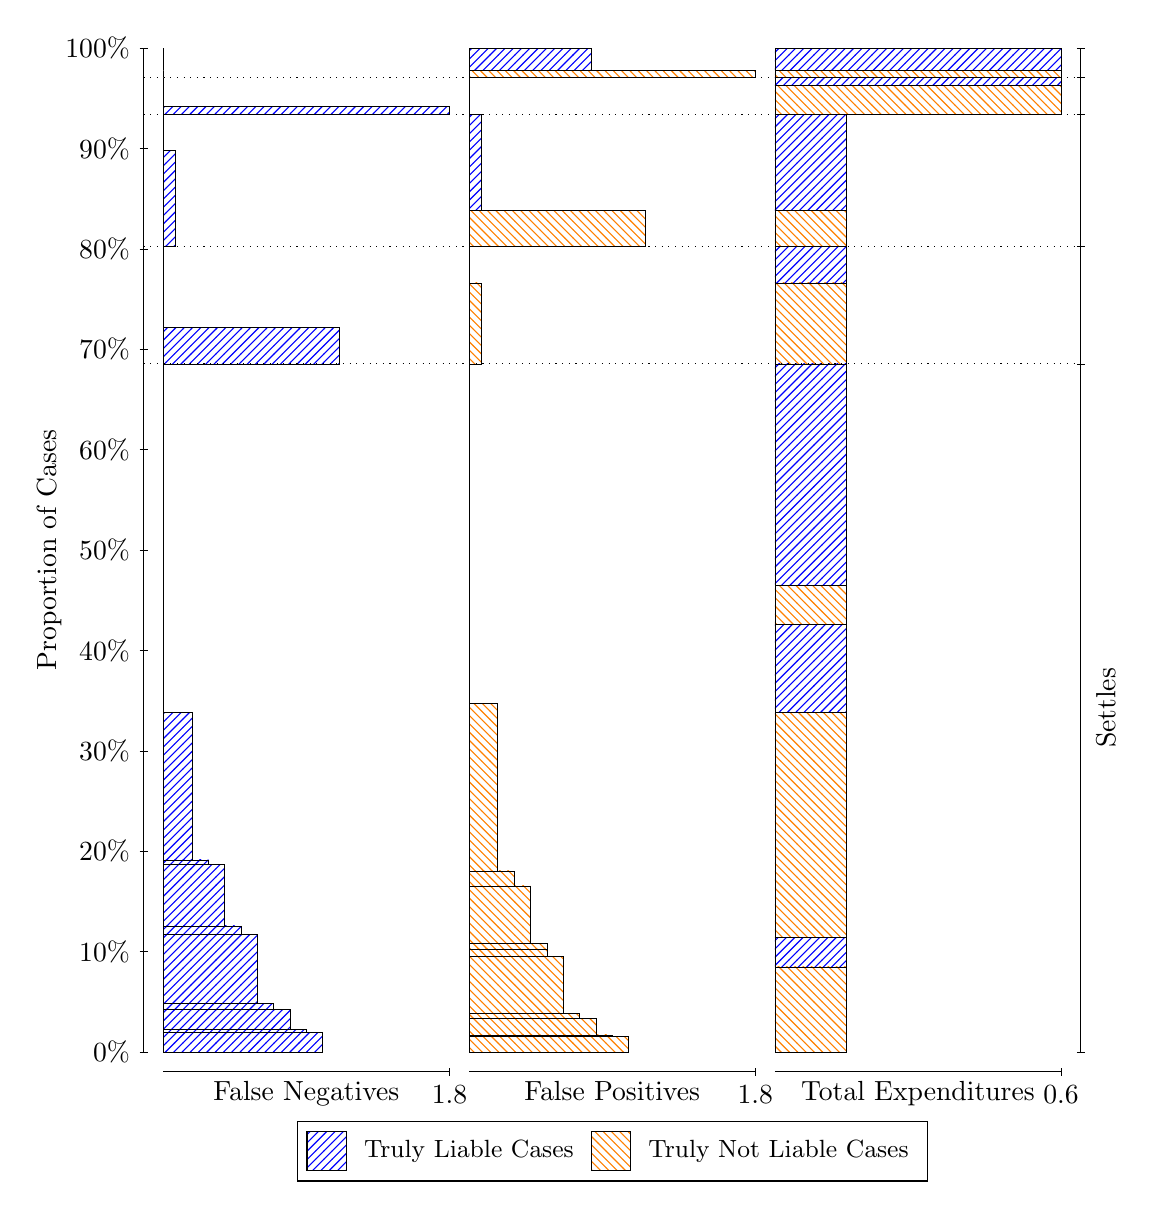
\begin{tikzpicture}
\draw[black, very thin] (1.5,1.75) -- (1.5,14.5);
\node[rotate=90, anchor=center] at (0.3, 8.125) {Proportion of Cases};
\draw[black, very thin] (1.45,1.75) -- (1.55,1.75);
\node[anchor=east] at (1.45, 1.75) {0\%};
\draw[black, very thin] (1.45,3.025) -- (1.55,3.025);
\node[anchor=east] at (1.45, 3.025) {10\%};
\draw[black, very thin] (1.45,4.3) -- (1.55,4.3);
\node[anchor=east] at (1.45, 4.3) {20\%};
\draw[black, very thin] (1.45,5.575) -- (1.55,5.575);
\node[anchor=east] at (1.45, 5.575) {30\%};
\draw[black, very thin] (1.45,6.85) -- (1.55,6.85);
\node[anchor=east] at (1.45, 6.85) {40\%};
\draw[black, very thin] (1.45,8.125) -- (1.55,8.125);
\node[anchor=east] at (1.45, 8.125) {50\%};
\draw[black, very thin] (1.45,9.4) -- (1.55,9.4);
\node[anchor=east] at (1.45, 9.4) {60\%};
\draw[black, very thin] (1.45,10.675) -- (1.55,10.675);
\node[anchor=east] at (1.45, 10.675) {70\%};
\draw[black, very thin] (1.45,11.95) -- (1.55,11.95);
\node[anchor=east] at (1.45, 11.95) {80\%};
\draw[black, very thin] (1.45,13.225) -- (1.55,13.225);
\node[anchor=east] at (1.45, 13.225) {90\%};
\draw[black, very thin] (1.45,14.5) -- (1.55,14.5);
\node[anchor=east] at (1.45, 14.5) {100\%};

\draw[black, very thin] (13.4,1.75) -- (13.4,14.5);
\draw[black, very thin] (13.35,1.75) -- (13.45,1.75);
\node[anchor=west] at (13.35, 1.75) {};
\draw[black, very thin] (13.35,10.489) -- (13.45,10.489);
\node[anchor=west] at (13.35, 10.489) {};
\draw[black, very thin] (13.35,11.983) -- (13.45,11.983);
\node[anchor=west] at (13.35, 11.983) {};
\draw[black, very thin] (13.35,13.66) -- (13.45,13.66);
\node[anchor=west] at (13.35, 13.66) {};
\draw[black, very thin] (13.35,14.123) -- (13.45,14.123);
\node[anchor=west] at (13.35, 14.123) {};
\draw[black, very thin] (13.35,14.5) -- (13.45,14.5);
\node[anchor=west] at (13.35, 14.5) {};

\draw[black, very thin, pattern color=blue, pattern=north east lines] (1.75,1.75) rectangle (3.7743,1.9988);
\draw[black, very thin, pattern color=blue, pattern=north east lines] (1.75,1.9988) rectangle (3.5667,2.0347);
\draw[black, very thin, pattern color=blue, pattern=north east lines] (1.75,2.0347) rectangle (3.359,2.2919);
\draw[black, very thin, pattern color=blue, pattern=north east lines] (1.75,2.2919) rectangle (3.1514,2.3709);
\draw[black, very thin, pattern color=blue, pattern=north east lines] (1.75,2.3709) rectangle (2.9438,3.2427);
\draw[black, very thin, pattern color=blue, pattern=north east lines] (1.75,3.2427) rectangle (2.7362,3.3515);
\draw[black, very thin, pattern color=blue, pattern=north east lines] (1.75,3.3515) rectangle (2.5286,4.137);
\draw[black, very thin, pattern color=blue, pattern=north east lines] (1.75,4.137) rectangle (2.321,4.1883);
\draw[black, very thin, pattern color=blue, pattern=north east lines] (1.75,4.1883) rectangle (2.1133,6.06);
\draw[black, very thin, pattern color=orange, pattern=north west lines] (1.75,6.06) rectangle (1.75,10.489);
\draw[black, very thin, pattern color=blue, pattern=north east lines] (1.75,10.489) rectangle (3.9819,10.955);
\draw[black, very thin, pattern color=orange, pattern=north west lines] (1.75,10.955) rectangle (1.75,11.983);
\draw[black, very thin, pattern color=blue, pattern=north east lines] (1.75,11.983) rectangle (1.9057,13.204);
\draw[black, very thin, pattern color=orange, pattern=north west lines] (1.75,13.204) rectangle (1.75,13.66);
\draw[black, very thin, pattern color=blue, pattern=north east lines] (1.75,13.66) rectangle (5.3833,13.754);
\draw[black, very thin, pattern color=orange, pattern=north west lines] (1.75,13.754) rectangle (1.75,14.123);
\draw[black, very thin, pattern color=orange, pattern=north west lines] (1.75,14.123) rectangle (1.75,14.216);
\draw[black, very thin, pattern color=blue, pattern=north east lines] (1.75,14.216) rectangle (1.75,14.5);
\draw[black, very thin, pattern color=orange, pattern=north west lines] (5.6333,1.75) rectangle (7.6576,1.9507);
\draw[black, very thin, pattern color=orange, pattern=north west lines] (5.6333,1.9507) rectangle (7.45,1.9665);
\draw[black, very thin, pattern color=orange, pattern=north west lines] (5.6333,1.9665) rectangle (7.2424,2.1763);
\draw[black, very thin, pattern color=orange, pattern=north west lines] (5.6333,2.1763) rectangle (7.0348,2.2418);
\draw[black, very thin, pattern color=orange, pattern=north west lines] (5.6333,2.2418) rectangle (6.8271,2.9675);
\draw[black, very thin, pattern color=orange, pattern=north west lines] (5.6333,2.9675) rectangle (6.6195,3.0601);
\draw[black, very thin, pattern color=orange, pattern=north west lines] (5.6333,3.0601) rectangle (6.6195,3.128);
\draw[black, very thin, pattern color=orange, pattern=north west lines] (5.6333,3.128) rectangle (6.4119,3.8605);
\draw[black, very thin, pattern color=orange, pattern=north west lines] (5.6333,3.8605) rectangle (6.2043,4.0485);
\draw[black, very thin, pattern color=orange, pattern=north west lines] (5.6333,4.0485) rectangle (5.9967,6.1786);
\draw[black, very thin, pattern color=blue, pattern=north east lines] (5.6333,6.1786) rectangle (5.6333,10.489);
\draw[black, very thin, pattern color=orange, pattern=north west lines] (5.6333,10.489) rectangle (5.789,11.517);
\draw[black, very thin, pattern color=blue, pattern=north east lines] (5.6333,11.517) rectangle (5.6333,11.983);
\draw[black, very thin, pattern color=orange, pattern=north west lines] (5.6333,11.983) rectangle (7.8652,12.44);
\draw[black, very thin, pattern color=blue, pattern=north east lines] (5.6333,12.44) rectangle (5.789,13.66);
\draw[black, very thin, pattern color=orange, pattern=north west lines] (5.6333,13.66) rectangle (5.6333,14.029);
\draw[black, very thin, pattern color=blue, pattern=north east lines] (5.6333,14.029) rectangle (5.6333,14.123);
\draw[black, very thin, pattern color=orange, pattern=north west lines] (5.6333,14.123) rectangle (9.2667,14.216);
\draw[black, very thin, pattern color=blue, pattern=north east lines] (5.6333,14.216) rectangle (7.1905,14.5);
\draw[black, very thin, pattern color=orange, pattern=north west lines] (9.5167,1.75) rectangle (10.425,2.8309);
\draw[black, very thin, pattern color=blue, pattern=north east lines] (9.5167,2.8309) rectangle (10.425,3.2031);
\draw[black, very thin, pattern color=orange, pattern=north west lines] (9.5167,3.2031) rectangle (10.425,6.0589);
\draw[black, very thin, pattern color=blue, pattern=north east lines] (9.5167,6.0589) rectangle (10.425,7.1795);
\draw[black, very thin, pattern color=orange, pattern=north west lines] (9.5167,7.1795) rectangle (10.425,7.6713);
\draw[black, very thin, pattern color=blue, pattern=north east lines] (9.5167,7.6713) rectangle (10.425,10.489);
\draw[black, very thin, pattern color=orange, pattern=north west lines] (9.5167,10.489) rectangle (10.425,11.517);
\draw[black, very thin, pattern color=blue, pattern=north east lines] (9.5167,11.517) rectangle (10.425,11.983);
\draw[black, very thin, pattern color=orange, pattern=north west lines] (9.5167,11.983) rectangle (10.425,12.44);
\draw[black, very thin, pattern color=blue, pattern=north east lines] (9.5167,12.44) rectangle (10.425,13.66);
\draw[black, very thin, pattern color=orange, pattern=north west lines] (9.5167,13.66) rectangle (13.15,14.029);
\draw[black, very thin, pattern color=blue, pattern=north east lines] (9.5167,14.029) rectangle (13.15,14.123);
\draw[black, very thin, pattern color=orange, pattern=north west lines] (9.5167,14.123) rectangle (13.15,14.216);
\draw[black, very thin, pattern color=blue, pattern=north east lines] (9.5167,14.216) rectangle (13.15,14.5);
\draw[black, dotted] (1.5,10.489) -- (13.4,10.489);
\draw[black, dotted] (1.5,11.983) -- (13.4,11.983);
\draw[black, dotted] (1.5,13.66) -- (13.4,13.66);
\draw[black, dotted] (1.5,14.123) -- (13.4,14.123);
\draw[black, very thin] (1.75,1.5) -- (5.3833,1.5);
\node[anchor=north] at (3.5667, 1.5) {False Negatives};
\draw[black, very thin] (5.3833,1.45) -- (5.3833,1.55);
\node[anchor=north] at (5.3833, 1.45) {1.8};

\draw[black, very thin] (5.6333,1.5) -- (9.2667,1.5);
\node[anchor=north] at (7.45, 1.5) {False Positives};
\draw[black, very thin] (9.2667,1.45) -- (9.2667,1.55);
\node[anchor=north] at (9.2667, 1.45) {1.8};

\draw[black, very thin] (9.5167,1.5) -- (13.15,1.5);
\node[anchor=north] at (11.333, 1.5) {Total Expenditures};
\draw[black, very thin] (13.15,1.45) -- (13.15,1.55);
\node[anchor=north] at (13.15, 1.45) {0.6};

\node[black, centered, rotate=90] at (13.72, 6.1193) {Settles};





\draw (7.449999999999999,1.5) node[draw=none] (baseCoordinate) {};
\begin{scope}[align=center]
        \matrix[scale=0.5, draw=black, below=0.5cm of baseCoordinate, nodes={draw}, column sep=0.1cm]{
            \node[rectangle, draw, minimum width=0.5cm, minimum height=0.5cm, pattern=north east lines, pattern color=blue] {}; &
            \node[draw=none, font=\small] (B) {Truly Liable Cases}; &
            \node[rectangle, draw, minimum width=0.5cm, minimum height=0.5cm, pattern=north west lines, pattern color=orange] {}; &
            \node[draw=none, font=\small] (B) {Truly Not Liable Cases}; \\
            };
\end{scope}

\end{tikzpicture}
\end{document}